\section{Experiments and Results}
\label{sec:experiments-and-results}

\subsection{Expert Survey: Indistinguishability of Synthetic Images}
\label{subsec:expert-survey:-indistinguishability-of-synthetic-images}
The expert survey results revealed a striking inability of microscopy experts to consistently distinguish synthetic brightfield microscopy images generated by our diffusion model from real images.
The overall classification accuracy all 11 participants and 30 images was remarkably close to chance level, reaching only 50\%.
This near-random performance strongly indicates the high degree of realism achieved by our synthetic image generation approach.
Figure~\ref{fig:conf_matrix} presents the normalized confusion matrix, visually demonstrating the balanced distribution of correct and incorrect classifications for both real and generated images.
Individual image accuracies varied significantly, ranging from approximately 18\% to 90\%, highlighting the inherent variability within both real and synthetic image sets and the complexity of the discrimination task.
Analysis of expert explanations revealed that experts considered subtle image features related to cell appearance, background texture, edge clarity, and perceived noise or artifacts when attempting to differentiate the images.
Prominent terms like ``cell,'' ``background,'' and ``edge'' indicate a focus on core microscopy image components, while terms such as ``pattern,'' ``perfect,'' ``artifacts,'' ``blurry,'' and ``contrast'' suggested that experts were searching for subtle imperfections or stylistic inconsistencies that might betray a synthetic origin.
However, these cues proved unreliable, ultimately leading to the near-chance level classification accuracy and underscoring the perceptual realism of our diffusion-generated brightfield microscopy images.

\begin{figure}[t]
    \centering
    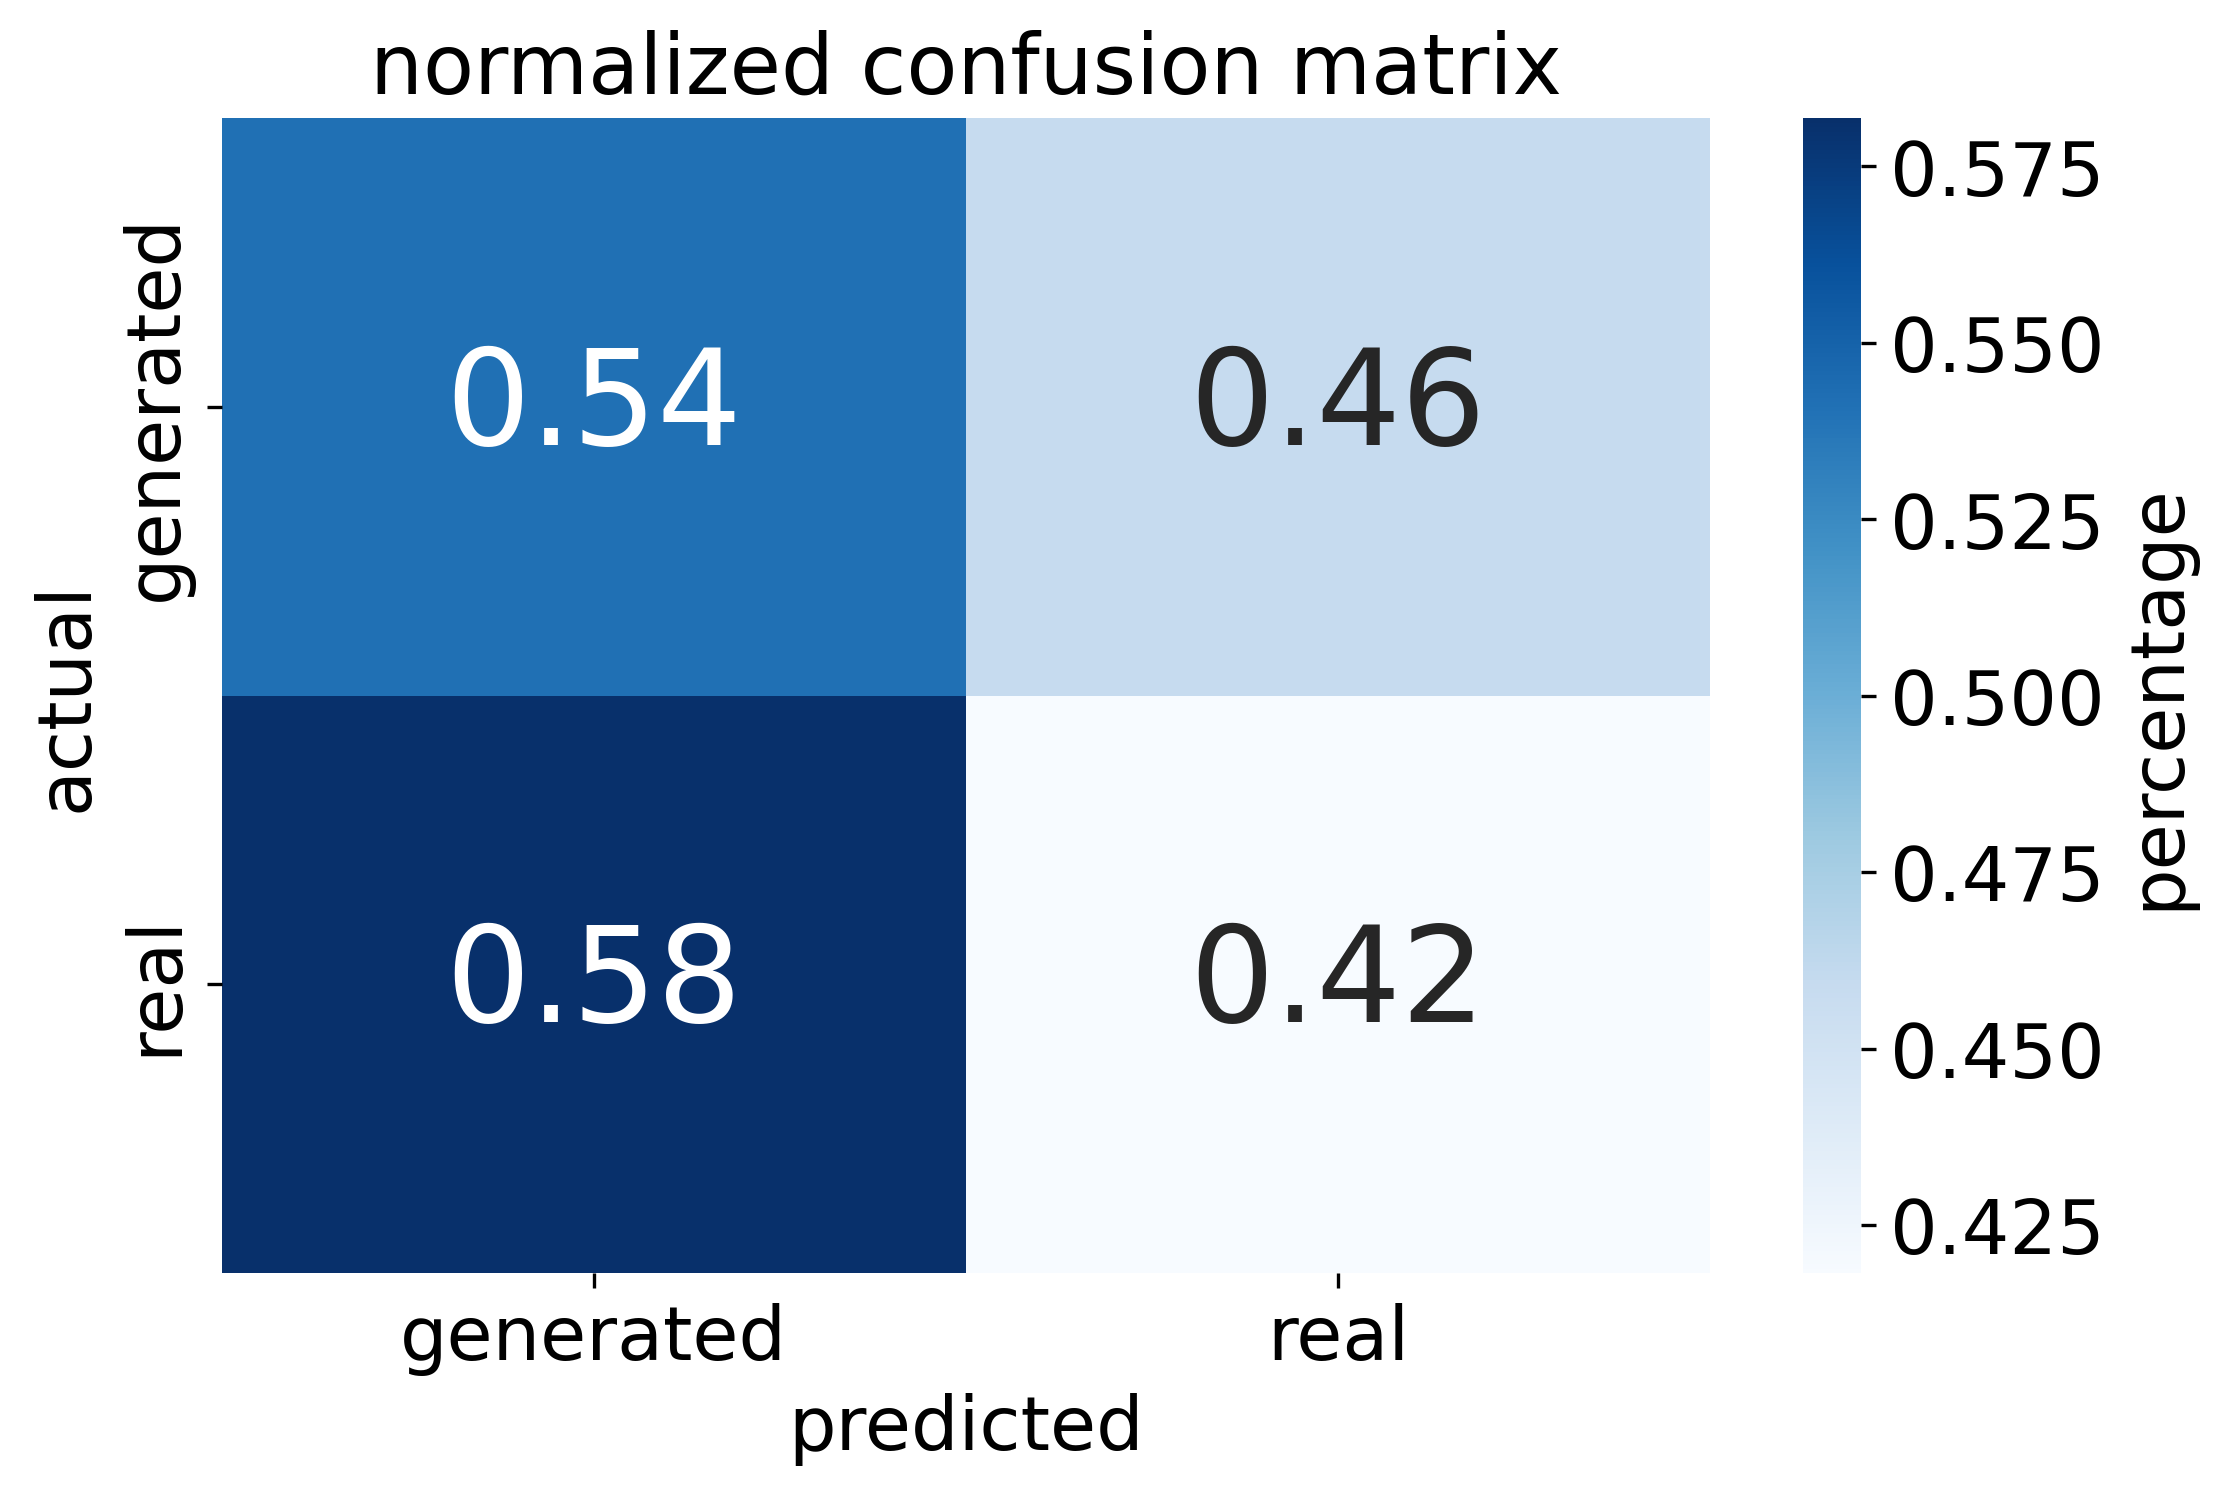
\includegraphics[width=0.75\linewidth]{images/norm_confusion_matrix}
    \caption{Normalized confusion matrix of expert survey classifications. Overall accuracy is approximately 50\%, demonstrating the significant difficulty for experts in distinguishing real and synthetic brightfield microscopy images.}
    \label{fig:conf_matrix}
\end{figure}

\subsection{Object Detection Performance}
\label{subsec:object-detection-performance}
Table~\ref{tab:model-performances} summarizes the object detection performance, presenting mAP metrics for all trained models across the seven datasets.
Analyzing mAP\@50, we observe that models trained with synthetic data replacing parts of the real data (\textit{scc\_10}, \textit{scc\_30}, \textit{scc\_50}) achieve comparable, and in some cases, improved performance compared to models trained solely on real data (\textit{scc\_real}).
Specifically, the YOLOv8s model trained on the \textit{scc\_30} dataset achieved a mAP\@50 of 0.9043, exceeding the 0.8947 achieved by the same model trained on the \textit{scc\_real} dataset.
Similarly, the RT-DETR-l model trained on the \textit{scc\_10} dataset reached a mAP\@50 of 0.9147, outperforming the 0.9146 achieved on the \textit{scc\_real} dataset.
However, when examining performance at higher IoU thresholds, specifically mAP\@75 and mAP\@50:95, a subtle trend of performance decrease emerges for models trained with increasing proportions of replaced synthetic data.
This trend is more pronounced for the RT-DETR models, indicating a potentially greater sensitivity of transformer-based architectures to the characteristics of synthetic data.

Continuing the analysis of object detection performance, we turn on the datasets where synthetic images were \textbf{added} to the real training data (\textit{scc\_add\_10}, \textit{scc\_add\_30}, \textit{scc\_add\_50}).
Examining mAP\@50 in Table~\ref{tab:model-performances}, we observe that models trained on these augmented datasets generally maintain a high level of performance, comparable to the baseline performance achieved with the \textit{scc\_real} dataset as well.
For instance, the YOLOv8s model shows a consistent mAP@50 around 0.8949-0.8952 across \textit{scc\_add\_10}, \textit{scc\_add\_30}, and \textit{scc\_add\_50}, similar to the 0.8947 of \textit{scc\_real}.
Notably, the YOLOv8m model achieves a mAP@50 of 0.9034 on \textit{scc\_add\_30}, closely matching the 0.9038 of the \textit{scc\_real} baseline.
The larger models, YOLOv8x, YOLOv9c, and YOLOv9e, also exhibit this trend of maintained high mAP@50 when trained with added synthetic data, suggesting that supplementing real data with synthetic images does not degrade the detection accuracy at this IoU threshold.

When considering the more stringent mAP@75 metric, we see a different pattern of maintained performance with added synthetic data compared to the replacement datasets.
In several instances, models trained on \textit{scc\_add\_30} even achieve slightly improved mAP@75 scores compared to the \textit{scc\_real} dataset.
For example, YOLOv8s reaches 0.8115 on \textit{scc\_add\_30} versus 0.8095 on \textit{scc\_real}, and YOLOv8m achieves 0.8224 on \textit{scc\_add\_30} compared to 0.8203 on \textit{scc\_real}.
This marginal improvement is also seen in YOLOv8x and YOLOv9c models on \textit{scc\_add\_30}.
Looking at the mAP@50:95 metric, only the YOLOv9e model trained on \textit{scc\_add\_50} achieves a higher score than the \textit{scc\_real} baseline, with a value of 0.6651 compared to 0.6629.

Generally, all models that were trained with replaced synthetic data augmentation maintained or achieved similar performance (less than 2\% difference) throughout the different datasets and IoU thresholds.
When it comes to models trained with added synthetic data, the performance was also maintained or slightly improved, particularly at lower IoU thresholds, with the exception of the RT-DETR models that showed a more pronounced sensitivity to the synthetic data proportion, achieving a
decreased performance of up to 5\% with the \textit{scc\_add\_50} dataset at more stringent IoU thresholds.
These results suggest that synthetic data augmentation can mostly maintain or even enhance detection performance at lower IoU thresholds, potentially due to increased data variability, dataset size and improved model robustness.

Qualitative assessment of sample detections revealed that all models, including those trained with synthetic data, generally performed well in detecting cells under the conditions proposed by the test split, including overlapping cells and cells at image boundaries.
However, subtle differences in detection precision and confidence scores were observed, especially for the transformer-based models, warranting further investigation into the fine-grained impact of synthetic data on model behavior.
\begin{table}[h!]
    \centering
    \caption{Detailed comparison of the performance metrics for all evaluated models across the different training datasets.}
    \label{tab:model-performances}
    \resizebox{\linewidth}{!}{%
    \begin{tabular}{l|l|c|c|c}
        \toprule
        Model                         & Dataset                 & mAP @50                    & mAP @75                    & mAP @50:95                 \\
        \midrule
        \multirow[t]{7}{*}{YOLOv8s}   & \textit{scc\_real}      & 0.8947                     & 0.8095                     & \cellcolor{blue!10}0.6557  \\
                                      & \textit{scc\_10}        & 0.8941                     & 0.8053                     & 0.6470                     \\
                                      & \textit{scc\_30}        & \cellcolor{blue!10}0.9043  & 0.8079                     & 0.6448                     \\
                                      & \textit{scc\_50}        & 0.8932                     & 0.7891                     & 0.6325                     \\
                                      & \textit{scc\_add\_10}   & 0.8949                     & 0.8068                     & 0.6502                     \\
                                      & \textit{scc\_add\_30}   & 0.8952                     & \cellcolor{blue!10}0.8115  & 0.6536                     \\
                                      & \textit{scc\_add\_50}   & 0.8940                     & 0.8100                     & 0.6514                     \\
        \midrule
        \multirow[t]{7}{*}{YOLOv8m}   & \textit{scc\_real}      & \cellcolor{blue!10}0.9038  & 0.8203                     & \cellcolor{blue!10}0.6637  \\
                                      & \textit{scc\_10}        & 0.9035                     & 0.8093                     & 0.6558                     \\
                                      & \textit{scc\_30}        & 0.8945                     & 0.8076                     & 0.6462                     \\
                                      & \textit{scc\_50}        & 0.8930                     & 0.8040                     & 0.6456                     \\
                                      & \textit{scc\_add\_10}   & 0.8943                     & 0.8088                     & 0.6550                     \\
                                      & \textit{scc\_add\_30}   & 0.9034                     & \cellcolor{blue!10}0.8224  & 0.6606                     \\
                                      & \textit{scc\_add\_50}   & 0.8950                     & 0.8218                     & 0.6588                     \\
        \midrule
        \multirow[t]{7}{*}{YOLOv8x}   & \textit{scc\_real}      & \cellcolor{blue!10}0.9038  & 0.8120                     & \cellcolor{blue!10}0.6639  \\
                                      & \textit{scc\_10}        & 0.9032                     & 0.8055                     & 0.6531                     \\
                                      & \textit{scc\_30}        & 0.9031                     & 0.8085                     & 0.6549                     \\
                                      & \textit{scc\_50}        & 0.8935                     & 0.7961                     & 0.6425                     \\
                                      & \textit{scc\_add\_10}   & 0.8941                     & 0.8090                     & 0.6560                     \\
                                      & \textit{scc\_add\_30}   & 0.8942                     & \cellcolor{blue!10}0.8212  & \cellcolor{blue!10}0.6639  \\
                                      & \textit{scc\_add\_50}   & 0.8938                     & 0.8195                     & 0.6440                     \\
        \midrule
        \multirow[t]{7}{*}{YOLOv9c}   & \textit{scc\_real}      & \cellcolor{blue!10}0.9047  & 0.8215                     & \cellcolor{blue!10}0.6645  \\
                                      & \textit{scc\_10}        & 0.9042                     & 0.8070                     & 0.6531                     \\
                                      & \textit{scc\_30}        & 0.9042                     & 0.8106                     & 0.6568                     \\
                                      & \textit{scc\_50}        & 0.8935                     & 0.7951                     & 0.6422                     \\
                                      & \textit{scc\_add\_10}   & 0.8954                     & 0.8211                     & 0.6615                     \\
                                      & \textit{scc\_add\_30}   & 0.8952                     & \cellcolor{blue!10}0.8217  & 0.6605                     \\
                                      & \textit{scc\_add\_50}   & 0.8947                     & 0.8102                     & 0.6594                     \\
        \midrule
        \multirow[t]{7}{*}{YOLOv9e}   & \textit{scc\_real}      & 0.9037                     & 0.8201                     & 0.6629                     \\
                                      & \textit{scc\_10}        & \cellcolor{blue!10}0.9041  & 0.8141                     & 0.6650                     \\
                                      & \textit{scc\_30}        & 0.8946                     & 0.8069                     & 0.6485                     \\
                                      & \textit{scc\_50}        & 0.8938                     & 0.8037                     & 0.6453                     \\
                                      & \textit{scc\_add\_10}   & 0.8950                     & 0.8188                     & 0.6623                     \\
                                      & \textit{scc\_add\_30}   & 0.8952                     & \cellcolor{blue!10}0.8209  & 0.6638                     \\
                                      & \textit{scc\_add\_50}   & 0.9031                     & 0.8188                     & \cellcolor{blue!10}0.6651  \\
        \midrule
        \multirow[t]{7}{*}{RT-DETR-l} & \textit{scc\_real}      & 0.9146                     & \cellcolor{blue!10}0.8169  & \cellcolor{blue!10}0.6614  \\
                                      & \textit{scc\_10}        & \cellcolor{blue!10}0.9147  & 0.8071                     & 0.6574                     \\
                                      & \textit{scc\_30}        & 0.9017                     & 0.7780                     & 0.6240                     \\
                                      & \textit{scc\_50}        & 0.9036                     & 0.7843                     & 0.6298                     \\
                                      & \textit{scc\_add\_10}   & 0.9146                     & 0.8064                     & 0.6526                     \\
                                      & \textit{scc\_add\_30}   & 0.9043                     & 0.7962                     & 0.6457                     \\
                                      & \textit{scc\_add\_50}   & 0.9036                     & 0.7932                     & 0.6372                     \\
        \midrule
        \multirow[t]{7}{*}{RT-DETR-x} & \textit{scc\_real}      & \cellcolor{blue!10}0.9164  & \cellcolor{blue!10}0.8257  & \cellcolor{blue!10}0.6748  \\
                                      & \textit{scc\_10}        & 0.9144                     & 0.8083                     & 0.6565                     \\
                                      & \textit{scc\_30}        & 0.9032                     & 0.7830                     & 0.6328                     \\
                                      & \textit{scc\_50}        & 0.9045                     & 0.8032                     & 0.6437                     \\
                                      & \textit{scc\_add\_10}   & 0.9133                     & 0.7991                     & 0.6459                     \\
                                      & \textit{scc\_add\_30}   & 0.9136                     & 0.8106                     & 0.6532                     \\
                                      & \textit{scc\_add\_50}   & 0.9012                     & 0.7682                     & 0.6203                     \\
        \bottomrule
    \end{tabular}%
    }
\end{table}



